\Chapter{RÉSULTAT}\label{sec:Theme2}

Les résultats sont présentés en commençant d’abord par décrire l’implémentation du modèle conceptuel d’automate présenté dans la sous-section~\ref{subsection_cadre_conceptuel}. Ensuite, ce sera présenté successivement les résultats propres à chacun des sous-objectifs décrits dans le chapitre~\ref{chapitre_methode}.

\section{Implémentation: du modèle conceptuel au modèle opérationnel}

L’implémentation de la machine (conceptuelle) est passée par la programmation manuelle d’une première interface et d’un premier noyau, en mettant à jour une version préliminaire de générateur basé sur une GUI\cite{bluiksnot_repo} en lui intégrant la capacité de générer du code à partir d’un module externe via son «hook» au moment de l’installation. La version à ce jour, ainsi que ses guides d’utilisation et ses scripts associés, sont disponibles sur le site de ERPLibre\footnote{\url{https://erplibre.ca}}.

L’interface permet l’interactivité avec un utilisateur ou le système-cible. L’interface est découplée en deux ensembles de méta-données: µ$_C^A$ et µ$_C^B$. µ$_C^B$ est l’ensemble qui paramétrise le passage de méta-données au code pour un module spécifique. µ$_C^A$ est l’ensemble qui paramétrise le passage de code aux méta-données tout en préparant un µ$_C^B$ adapté à ce module spécifique. Ce découplage a permis l’adaptation de l’interface au contexte de l’installation de modules sur une instance Odoo via des «hooks». Par la suite, un ensemble supplémentaire de méta-données, noté µ$_C^0$, a été dégagé de la programmation manuelle de versions successives de µ$_C^A$. µ$_C^0$ sert à initialiser une version de départ de µ$_C^A$.

Le noyau prend les paramètres issus de l’interface pour créer des méta-données, générer l’ensemble des fichiers des modules désirés (mode direct) et faire de la rétro-ingénierie (mode indirect) sur des modules existants.

\subsection{Développement et amélioration continue}

Dans la Figure~\ref{fig:dia_sequence_gc}, µ$_C^0$, µ$_C^A$, µ$_C^B$, C et M sont tous des modules installables sur Odoo. $M^i$ et $M^d$ sont des sections de code dans le module M. µ$_C^0$, µ$_C^A$ et µ$_C^B$ dépendent de M. µ$_C^A$, c’est les macro-méta-données, que µ$_C^B$, c’est les micro-méta-données.

\begin{figure}[htb]
\centering
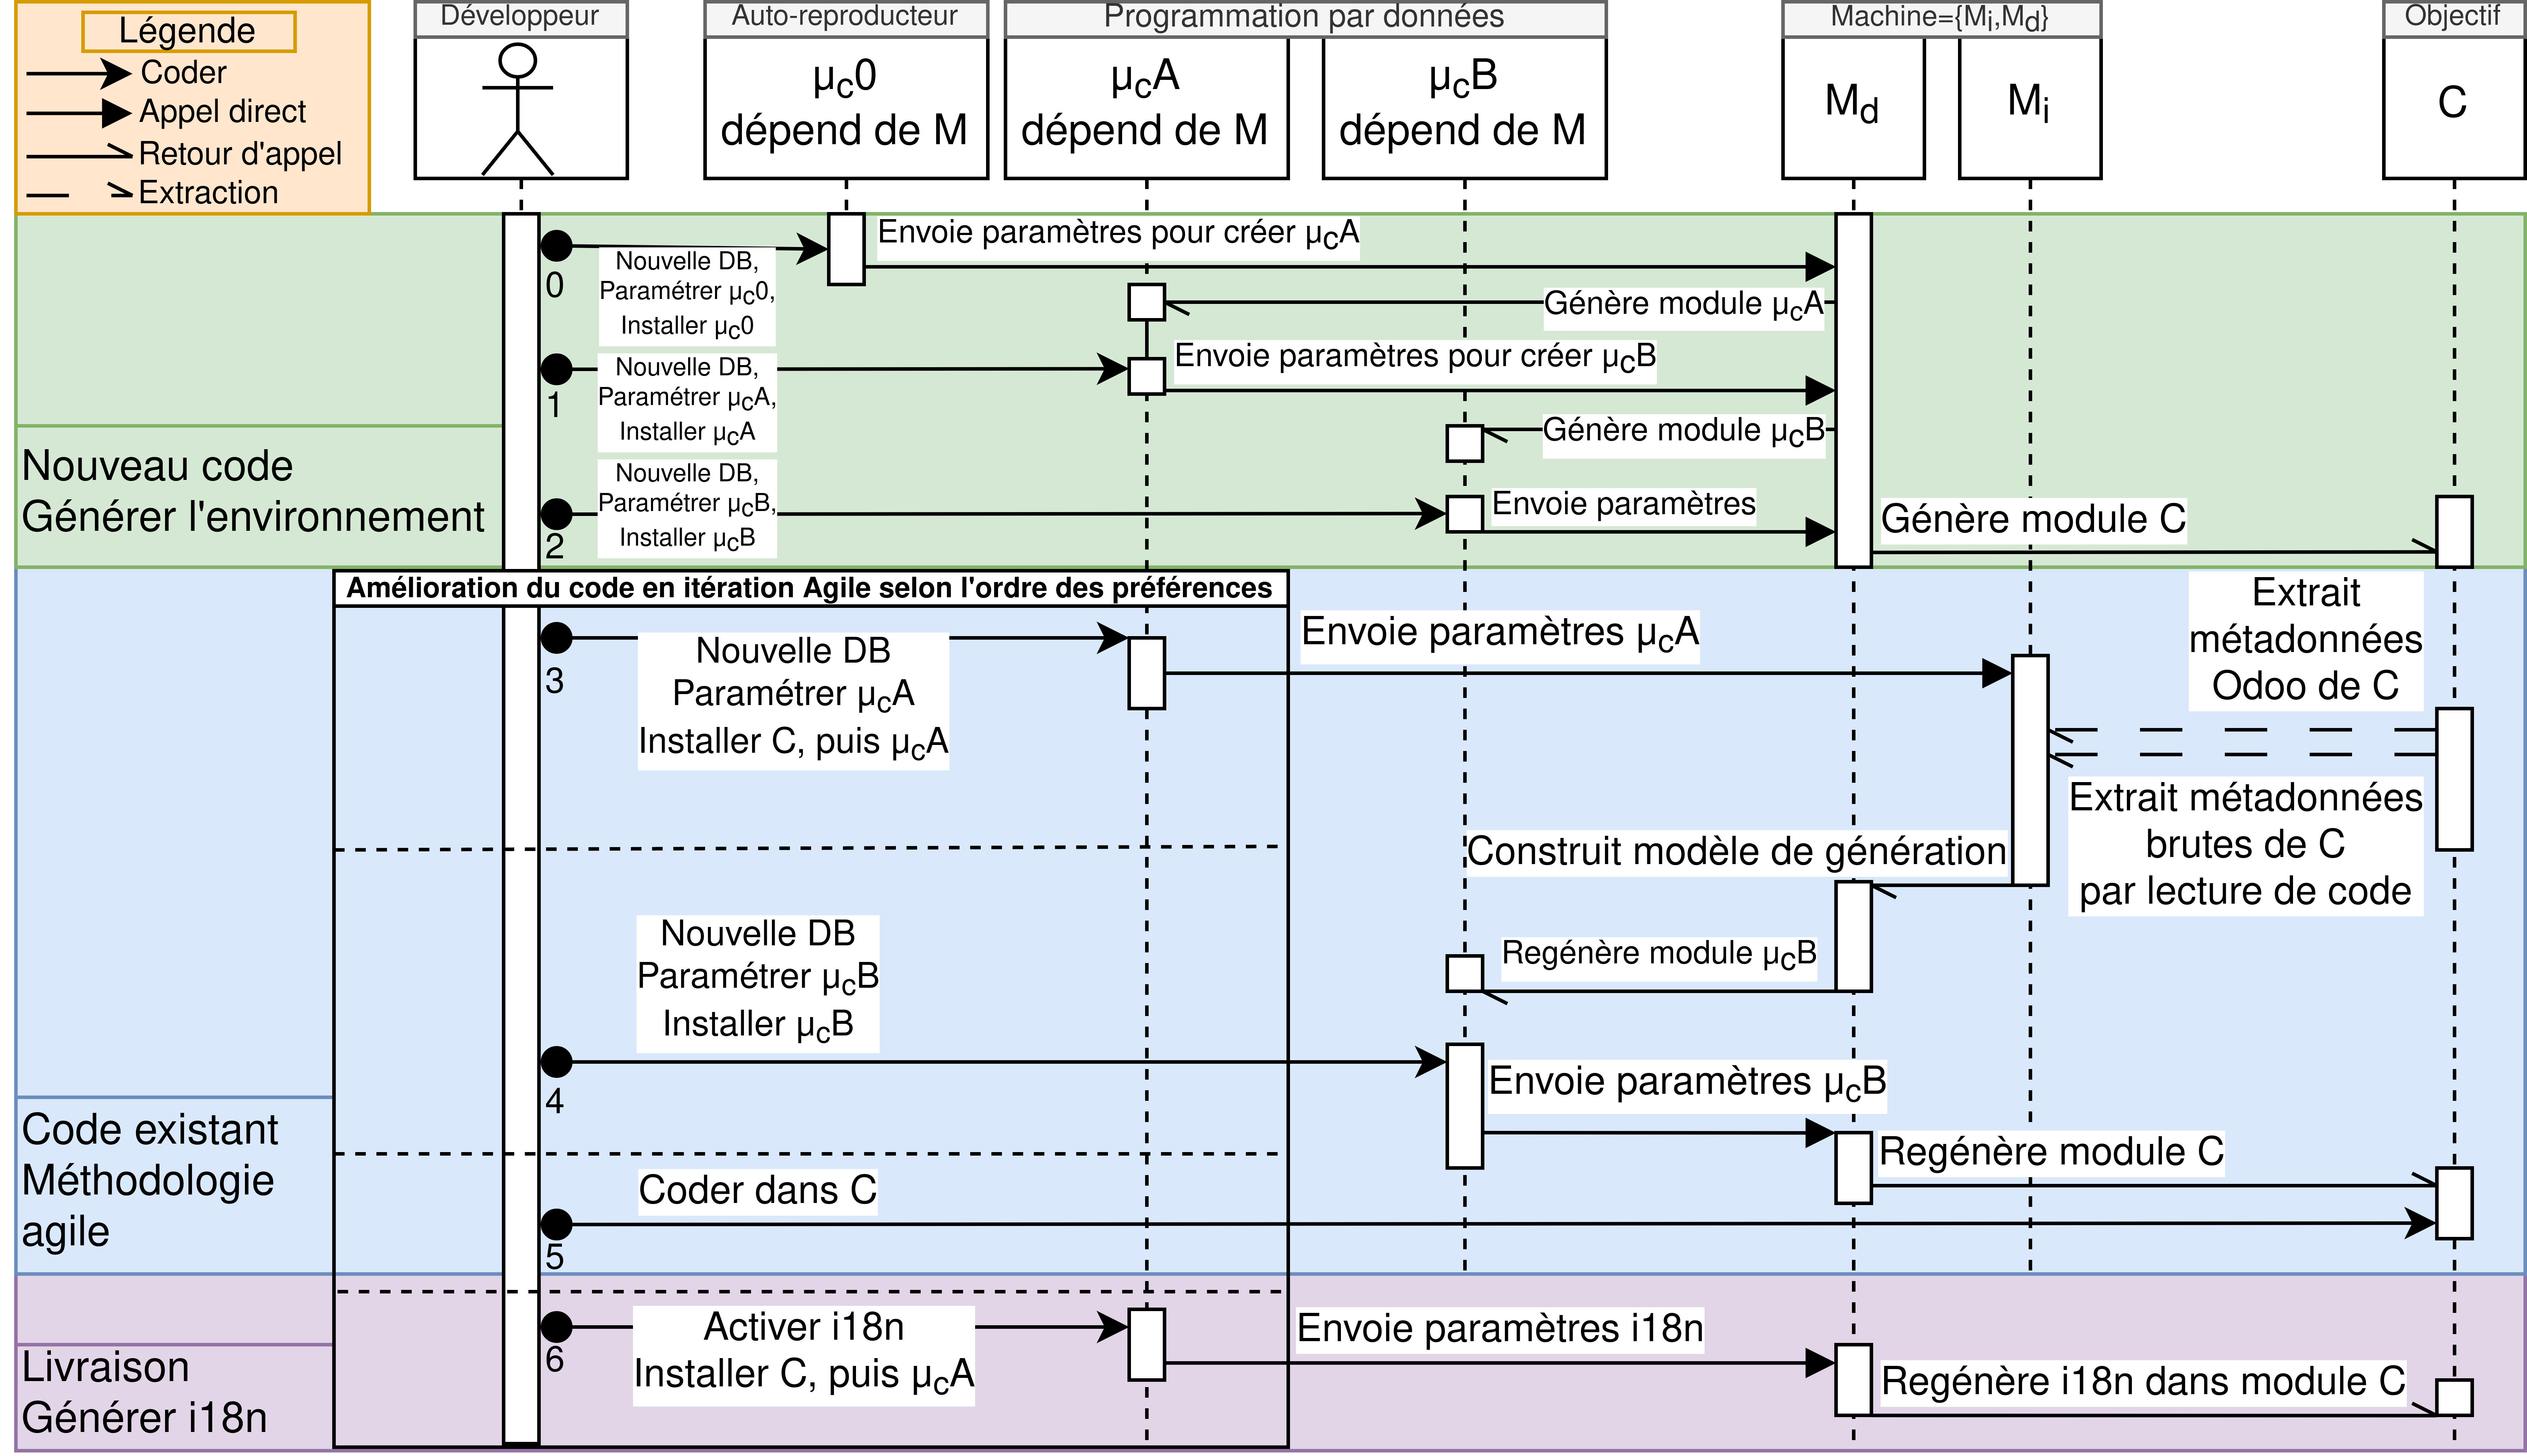
\includegraphics[width=6.535in]{images/code_generateur_erplibre_global_sequence.drawio.png}
\caption{Interaction du développeur avec le générateur de code}
\label{fig:dia_sequence_gc}
\end{figure}

Au départ d’un nouveau module code, µ$_C^0$ génère µ$_C^A$ qui génère µ$_C^B$ qui génère C. Il existe un script qui automatise un nouveau code, le développeur peut paramétrer le nom des modules et leurs emplacements. Ensuite, le développement commence en itération agile, les actions de 3 à 6 peuvent être exécutées dans l’ordre du choix du développeur.

% TODO expliquer raison/avantage de modifier soit µ$_C^A$, µ$_C^B$ ou le code directement.

Passer par l’étape 3 permet de mettre à jour l’étape 4 selon l’état du code via la rétro-ingénierie. Passer par l’étape 4 permet de mettre à jour le code selon le générateur. Il est possible de générer de nouvelles sections, comme la vue portail. Passer à l’étape 5 permet de personnaliser le code directement. Passer par l’étape 6 permet de mettre à jour le i18n de manière automatique.

La livraison sert à générer le i18n. C’est Odoo qui le génère, mais le générateur envoie les commandes, la liste des langues désirées à supporter et place les fichiers aux bons endroits dans le module. La raison pour laquelle c’est µ$_C^A$ qui doit le générer, c’est parce que le module doit être fini d’être généré et rechargé pour ensuite générer les langues, sinon ils sont corrompus par les traces de µ$_C^B$.

% TODO mettre dans discussion : Dans un contexte où l’ingénierie et la rétro-ingénierie serait parfaite, on n’aura pas besoin de mémoriser µ$_C^A$ et µ$_C^B$. Entre-temps, il y a une intervention humaine sur chacun de ces modules pour accélérer le développement. L’outil Git est utilisé pour faire des comparaisons entre les états d’itérations, seul ce qui est commité contient le bon contenu.

\subsection{Architecture}

La Figure~\ref{fig:dia_architecture_automate}, elle démontre un développeur qui utilise l'interface de la machine qui opère dans le noyau de la machine.

\begin{figure}[htb]
\centering
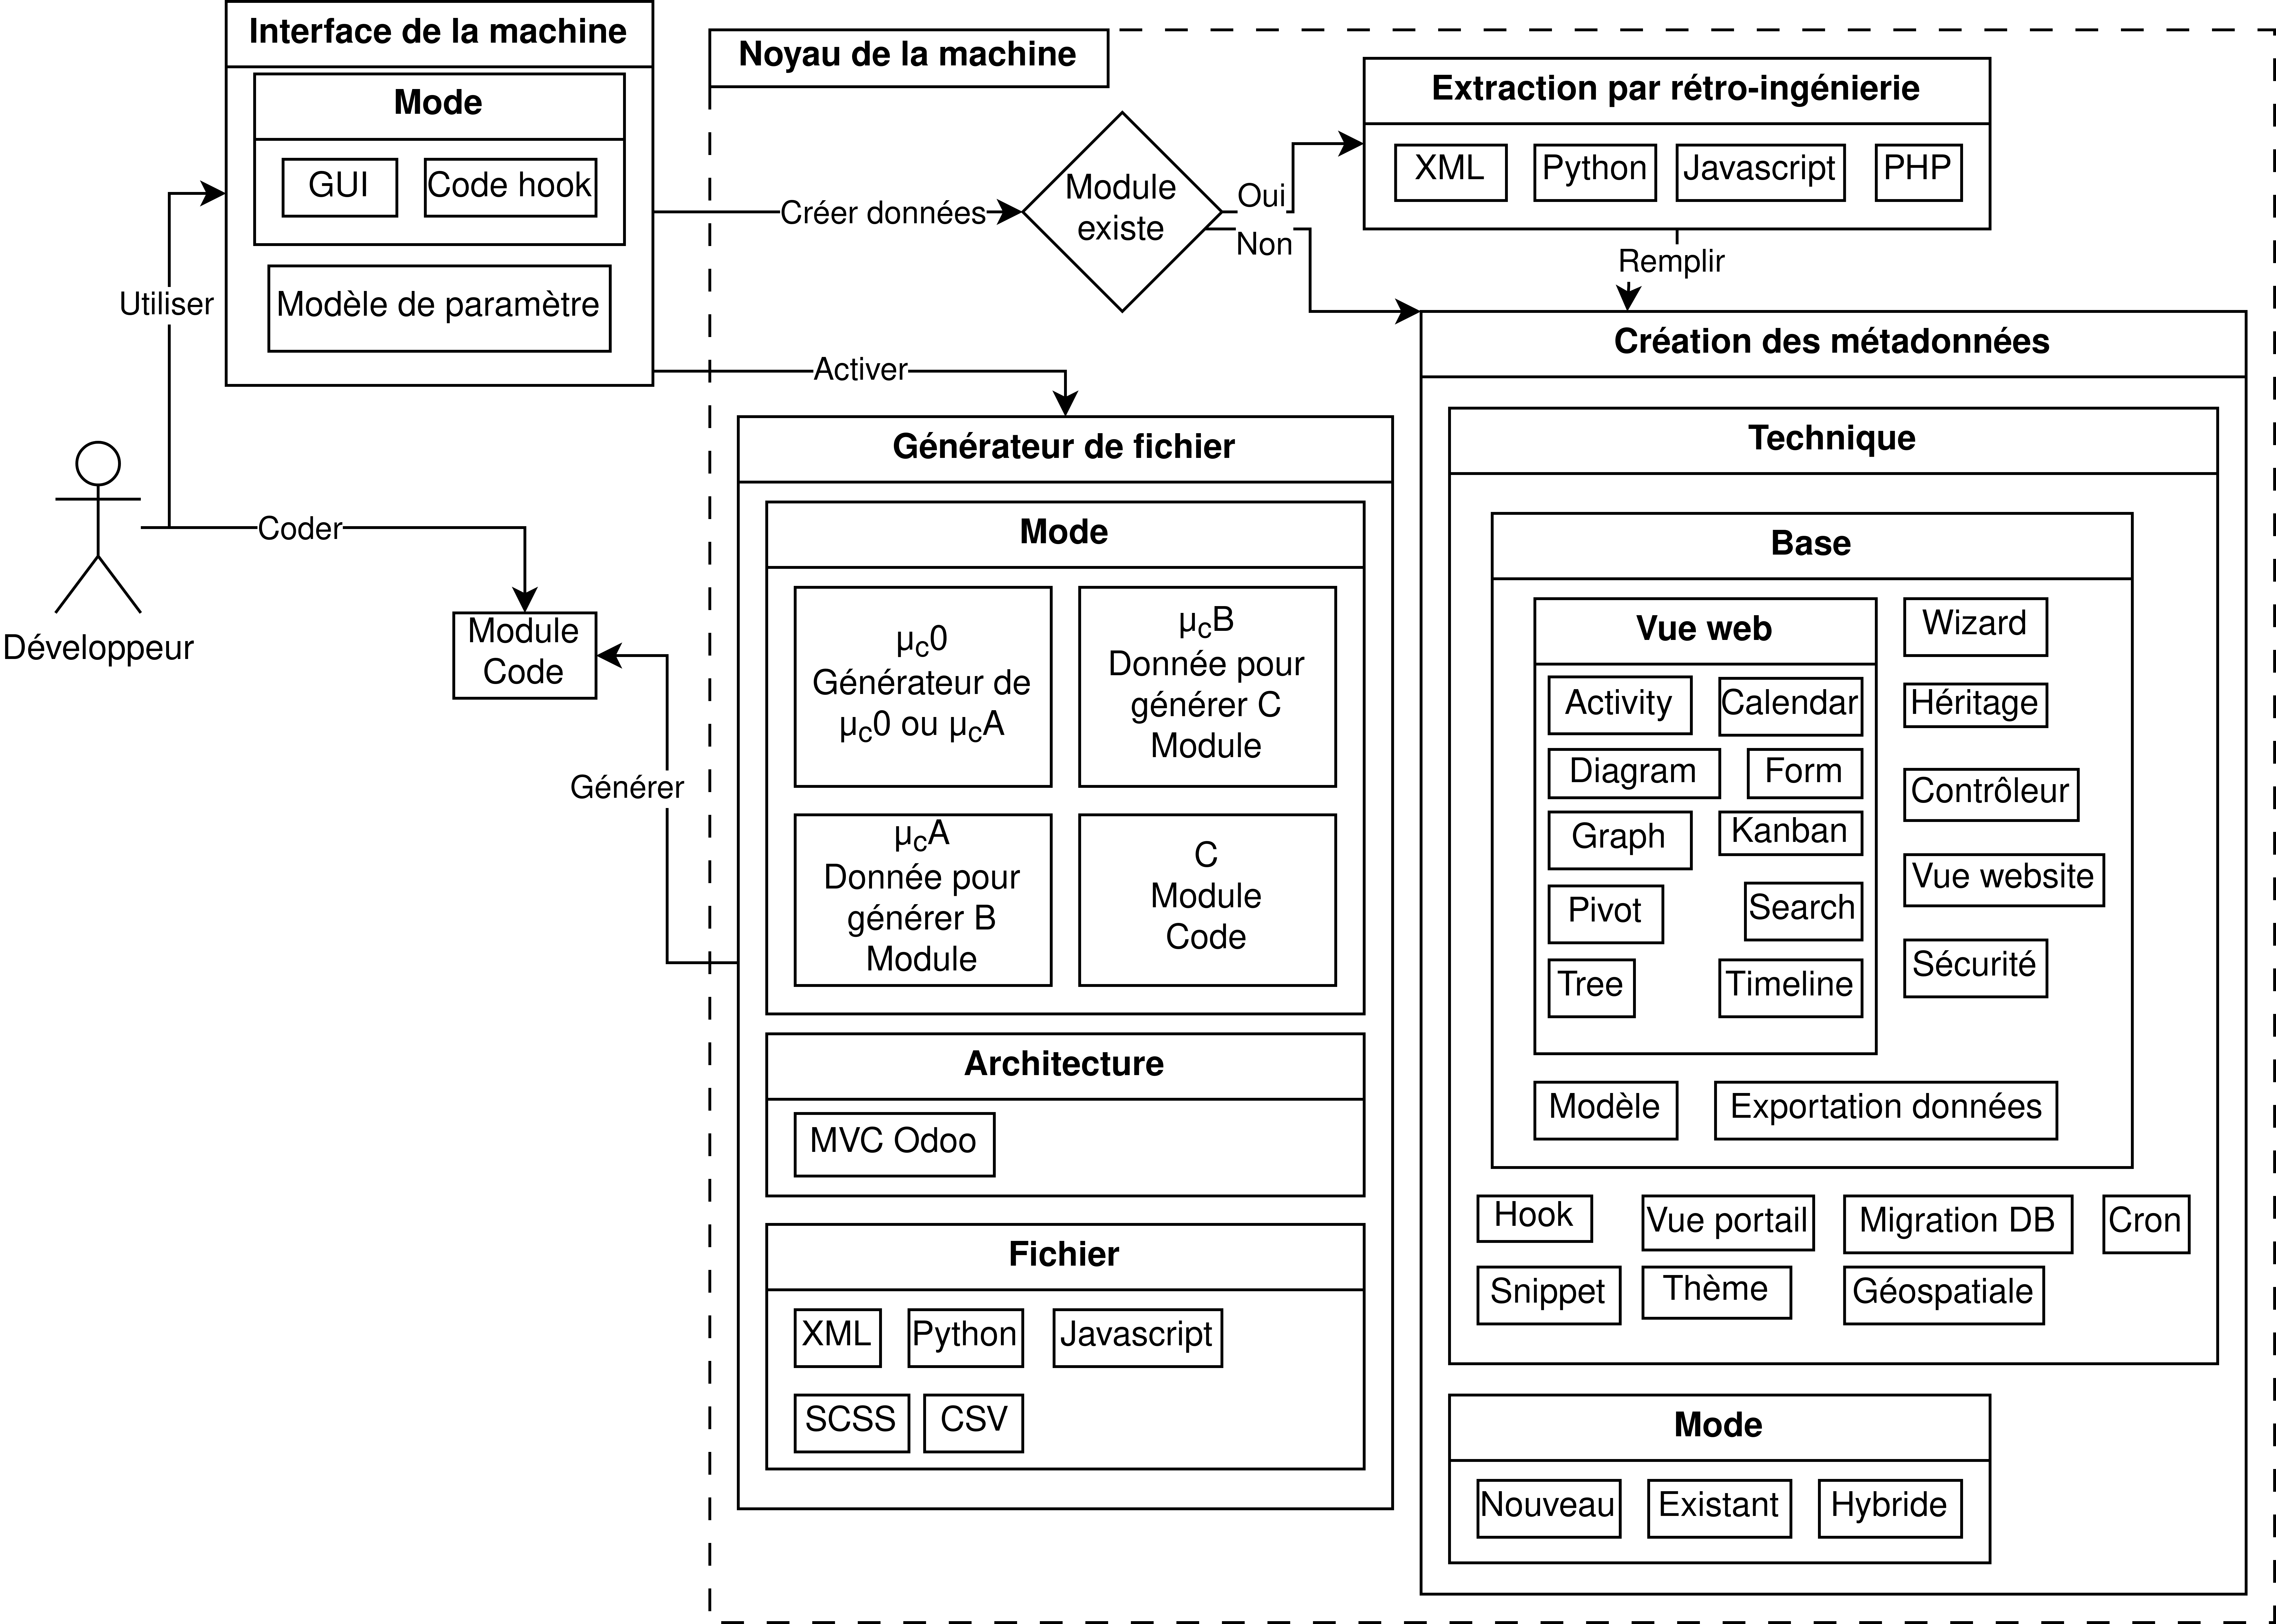
\includegraphics[width=6.535in]{images/architecture_machine.drawio.png}
\caption{Architecture de l'automate}
\label{fig:dia_architecture_automate}
\end{figure}

\begin{enumerate}
    \item L’interface machine permet à l’utilisateur de créer un modèle de données pour indiquer à la machine quelle opération effectuée avec leurs données associées. Plusieurs combinaisons, héritables, sont possibles selon les différentes techniques. De plus, c’est ici qu’on vient activer la génération de code.
    \item L’extraction par rétro-ingénierie permet de remplir le modèle de méta-données sans passer par la paramétrisation. Il extrait des informations qui ne sont pas accessibles dans le modèle de données d’Odoo sur le module.
    \item La création de méta-données se fait soit par l’utilisateur via la GUI ou le «Code Hook», il gère à la fois plusieurs techniques qui sont dans des modules. Le mode «nouveau» permet de créer de nouvelles données. Une fois qu’ils sont créés, c’est le mode «existant» qui est utilisé. Cependant le mode «hybride» permet d’écraser les données existantes en réactivant le mode «nouveau».
    \item Le générateur de fichier se fait activer par l’interface, mais il prend les méta-données pour faire sa génération selon le mode qu’il doit générer et l’architecture qu’il connaît. Il fait des liaisons entre les modèles et les vues en référence aux noms des champs de chaque modèle de données.
\end{enumerate}

Chacun de ces blocs de l’architecture est modulaire, chaque technique est héritable pour modifier le comportement et ajouter des liaisons pour permettre une génération de code au final.

La sécurité dépend du modèle. Le contrôleur dépend du modèle. La vue dépend du contrôleur et du modèle.

\subsection{Auto-générateur}

Représenté par µ$_C^0$, voir Annexe~\ref{annexe_cg_code_uc0}, c’est un auto-générateur! Au moment de son installation, il génère le même code que lui-même au même endroit dans le système de fichier. Une légère modification va créer une autre entité qui sera une déviation dans l’objectif de démarrer une chaîne.

C'est le module \texttt{M} qui contient les méta-données de µ$_C^0$. Ainsi, exécuter µ$_C^0$ devient un test de fonctionnalité et c'est un succès lorsqu'il n'y a pas de différence. Cependant sa programmation est actuellement spécifique à sa génération, aucun autre module n’a besoin de cette fonctionnalité unique.

% TODO TODO calcul code unique. HOW. Regarder le nombre de ligne exécuter avec ce module VS le nombre de ligne pour un autre module simple même type -> son µ$_C^A$ avec aucun modèle et un hook.
% TODO mettre référence vers le code

% Il pourrait être plus petit, faire appel à des méthodes extérieures. De plus, il pourrait y avoir moins de paramètre, on est pris entre la faciliter de paramétrer rapidement et la gestion de la lourdeur de beaucoup de paramètres. Présentement, la machine est limitée en fonctionnalité, mais plus que ça va avancer, plus il y aura de paramètres et il en aura trop pour tous les ajouter.

% TODO le terme chaine est nouveau, il faudrait le définir

L'auto-générateur est utilisé pour générer des µ$_C^A$ avec une légère modification dans les paramètres. Même s'il a la capacité de générer un µ$_C^B$, mieux vaut créer la chaîne proposé pour faire de l'amélioration continue.

\section{Résultats propres à SO-1}

\subsection{Génération par gabarit}

La génération par gabarit était déjà supportée dans la version initiale~\cite{bluiksnot_repo}, de plus, il y a eu des améliorations :
\begin{enumerate}
%TODO mettre en référence \footnote{\url{https://docs.python.org/3/whatsnew/3.6.html#pep-498-formatted-string-literals}}
    \item Utilisation des f-strings au lieu d'utiliser la fonction «format» de String.
    \item Utilisation de la bibliothèque Code-writer en Python\footnote{\url{https://pypi.org/project/code-writer/}}
    \item Utilisation de la bibliothèque lxml\footnote{\url{https://pypi.org/project/lxml/}}
\end{enumerate}

\subsection{MVC}

L’architecture MVC était déjà supportée dans la version initiale~\cite{bluiksnot_repo}, de plus, il y a eu des améliorations : 

\begin{enumerate}
% TODO define Wizard
 \item Ajout de bouton qui ouvre des «Wizard» pour générer les «Views», les «Models» et les «Controllers». Ainsi le développeur peut les configurer et demander de générer les méta-données associées.
    \begin{figure}[htb]
    \centering
    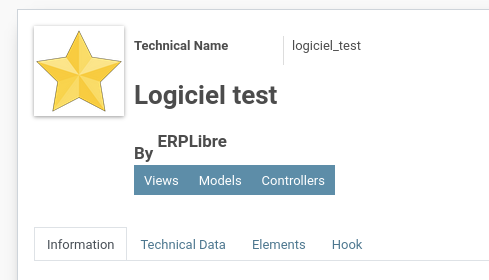
\includegraphics[width=3in]{images/GUI_MVC.png}
    \caption{Architecture de l'automate}
    \label{fig:dia_gui_mvc}
    \end{figure}
 \item Les règles de sécurité sont ajustées selon les configurations et personnalisables par la suite.
\end{enumerate}

\subsection{Générer un module à partir d’une base de données externes}

% Un module a été programmé pour suivre la technologie ETL
% TODO manque le load de https://fr.wikipedia.org/wiki/Extract-transform-load
% ça devient discussion

La migration de données à partir de \texttt{SQL} était déjà supporté dans la version initiale~\cite{bluiksnot_repo}, cependant il y a eu des améliorations : 

\begin{enumerate}
    \item Ajout de type de données, dont ceux utilisé par le projet Accorderie
    \item Ajout d'association entre les types de données et les différentes personnalisations de l’architecture Odoo
    \item Interface représentant la base de données avec les contrôleurs permettant la configuration de la migration sur le modèle de données désirés
    \item Gestion des interdépendances (A de B et B de A)
\end{enumerate}

\subsection{Génération de code par des données}

La capacité de prendre les données via les interfaces utilisateurs telles que la GUI et le «Code hook» est de la génération de code par des données. Cela permet de personnaliser pour obtenir un logiciel adapté à ce que l’utilisateur est capable d’exprimer.

L’automate est une machine qui grâce à son interface «code hook», il se fait commander par deux couches de méta-données paramétrable par l’humain. Les deux couches s’interfèrent entre eux pour permettre l’évolution de la fonctionnalité désirée.

% TODO diagramme de couche entrée de l’utilisateur et sortie des fonctionnalités.

\section{Résultats propres à SO-2}

\subsection {Extraction de code et reproduction}

De la macro et micro extraction a été réalisé avec plusieurs techniques combinées.

Pour pouvoir faire de la reproduction, il a suffit de faire de la macro extraction, c'est-à -dire faire une recherche dans toutes les classes pour copier le contenu de chaque méthode pour le transformer en méta-données et pouvoir faire l’opération direct de générer le code qui a été copié. L’utilisation de l’\texttt{AST} a servi à déterminer quelle ligne de code était à découper pour les recopier.

Cependant il était nécessaire dans certain contexte de faire de la micro extraction, comme : 
\begin{enumerate}
    \item L’extraction des noms des constantes, ils sont transformés en valeur lors de l’exécution;
    \item L’extraction des commentaires, qui n’est pas supporté dans la bibliothèque \texttt{AST} de Python 3.7;
    \item L’extraction des décorateurs;
    \item L’extraction des paramètres et nom des méthodes/fonctions;
    \item Les méta-informations d’un modèle (description, nom, etc.)
\end{enumerate}

De plus, les vues ont été extraites dans le but d'obtenir des méta-données spécifiques qui caractérise la reconstruction de la vue, ces données n’étaient pas accessibles dans les données d'Odoo.

Certaines informations ont été extraites dans le Javascript à l’aide de la bibliothèque «pyjsparser».

Pour l’extraction d'un projet externe d'une autre technologie, un extracteur de PHP a été développé via un «parser» de la communauté\footnote{\url{https://github.com/JameelNabbo/PHP-Parsers}}.

% TODO manque info sur le générateur de générateur de code
C'est en développent les techniques de génération de code qu'on réalise la reproduction. Un script a été développé pour accélérer l’écriture du générateur de code, ainsi un générateur de générateur de code. Ensuite le développeur peut le transformer légèrement pour prendre les paramètres des méta-données.

\subsection {Amélioration continue sur la génération}

Grâce à l’extraction des méta-données, dès que la technique de génération est bien développé avec les méta-données, le code est automatiquement généré avec des bonnes pratiques logicielles corrigeant automatiquement les problèmes.

L’intérêt de passer par Odoo pour lire le module valide déjà certains fonctionnements (par exemple : pas d’erreur de syntaxe dans le Python ou les \texttt{XML} étaient bien construits).

Ainsi, pour un module désiré, nous utilisons les outils pour générer µ$_C^A$ et µ$_C^B$, puis en avançant dans le développement, nous bouclons entre le 3 et 4 sur Figure~\ref{fig:dia_sequence_gc}.

\subsection {Test de validation de génération de codes}

Pour tester ce générateur de code, la technique du test de comparaisons des sorties de la génération a été utilisé. Pour procéder, un développeur valide via l'outil Git ce qui est commité\footnote{Un terme dans l'outil Git pour valider le code en créant un état dans l'historique.}. Ainsi, un script a été développé pour lancer en parallèle les tests et valider les différences de génération avec ce qui a été commité précédemment. Aucune différence est un succès.

Il y a plusieurs types de test : 
\begin{enumerate}
    \item Valider l’installation du module généré;
    \item Valider que µ$_C^B$ génère bien le module cible sans différence dans le code;
    \item Valider que µ$_C^A$ génère bien µ$_C^B$ sans différence dans le code;
    \item L’extraction des paramètres et nom des méthodes/fonctions;
    \item Valider que la migration d’une base de données \texttt{SQL} se fait sans différence dans le code.
\end{enumerate}

En exécutant tous les tests, voir annexe~\ref{annexe_test_generateur_code}, une couverture de 84\% est obtenu, tous les tests présents sont un succès, sauf ceux sur l’auto-générateur.

\subsection {Règles de codage standardisées}

Au moment de générer les fichiers, toutes les sorties textes sont traitées par des outils de mise en forme suivant des règles de codage standardisées.

Pour le Python, l’outil «black» est utilisé pour la mise en forme, suivant le standard \texttt{PEP8} avec «isort» pour réordonner les importations. «black» donne une mise en forme non naturel comparé à l’écriture de code pour un humain, cependant son résultat facilite la lecture et le suivi des différences pour les futurs ajouts.

Le Javascript, le HTML et le \texttt{XML} sont mises en forme avec l’outil «prettier».

De plus, le générateur force le déplacement des classes dans leur propre fichier respectif pour faire une classe par fichier.

Les champs pour chaque modèle sont déplacés en ordre alphabétique, mais le premier est celui qui est utilisé pour représenter le modèle\footnote{Référence à l'attribut «\_rec\_name»}.

\section{Résultats propres à SO-3}

\subsection{Classification des techniques développés}

En référence à la Figure~\ref{fig:dia_architecture_automate}, les techniques «Modèle», «Form», «Tree», «Contrôleur» et «Migration DB» étaient déjà implémentés dans la version initiale~\cite{bluiksnot_repo}, mais ils ont reçu des améliorations pour s’agencer aux autres techniques.

% TODO faire un diagramme des dépendances
Les techniques :
\begin{enumerate}
    \item Contrôleur;
    \item Cron;
    \item Exportation des données;
    \item Géospatiale (dépend de Modèle);
    \item Héritage;
    \item Hook;
    \item Migration DB\footnote{importation des données par DB};
    \item Modèle;
    \item Portal;
    \item Sécurité;
    \item Snippet;
    \item Thème;
    \item Vue web;
    \begin{enumerate}
        \item Activity;
        \item Calendar;
        \item Diagram;
        \item Form;
        \item Graph;
        \item Kanban;
        \item Pivot;
        \item Search;
        \item Timeline;
        \item Tree;
    \end{enumerate}
    \item «website\_leaflet» (dépend de Snippet et Géospatiale);
    \item Wizard;
\end{enumerate}

\subsection{Interface du générateur de code}

\paragraph{L'interface graphique}

 existait déjà dans la version initiale~\cite{bluiksnot_repo}, elle a été améliorée pour afficher plus d'informations par rapport aux développements. Elle sert à faciliter la paramétrisation du générateur de code. Elle n’a pas été priorisée et elle manque de fonctionnalité comparé à ce qui peut être supporté via la technique «code hooks» avec µ$_C^A$ et µ$_C^B$.

Ce qui fonctionne : 
\begin{enumerate}
    \item Créer module;
    \item Renommer un module;
    \item Ajouter des modèles, voir Annexe~\ref{annexe_cg_gui_model}, et des champs, voir Annexe~\ref{annexe_cg_gui_champs};
    \item Ajouter des menus;
    \item Ajouter la sécurité;
    \item Changer les icônes;
    \item Changer les informations sur les propriétés «manifest» du module;
    \item Ajouter du code, voir Annexe~\ref{annexe_cg_gui_code};
    \item Modification des «hooks», voir Annexe~\ref{annexe_cg_gui_hook};
    \item Etc.
\end{enumerate}

\paragraph{L'interface «code hook»}

% TODO on montre un exemple de code hook?

permettent d’accéder à la totalité des fonctionnalités de l’automate via µ$_C^A$ et µ$_C^B$, elles ont été utilisés pour toutes les démonstrations qui servent de test, elles contiennent la paramétrisation pour des modules désirés.

\section{Résultats propres à SO-4}

\subsection{Utilisation d’un conteneur Docker}

Puisque l’automate fait partie de ERPLibre, la version 1.5.0 contient les modules de génération de code. Le déploiement se fait rapidement en utilisant le logiciel Docker, le générateur de code permet l’utilisation de l’interface graphique pour générer des modules Odoo.

\section{Résultats propres à SO-5}

\subsection{Guide créer une communauté autour d’une technologie pour un réseau d’entraide libre}

Un guide hybride a été produit pour comprendre les aspects cités du démarrage d’un projet, de gestion d’une communauté autour d’un projet libre et des règles d'hébergement libres.

\subsection{Démarrage d’un projet}

Le guide du tableau~\ref{tab:demarrer_projet_7_etape} permet de démarrer rapidement un projet et s'assurer que les membres impliqués du réseau d'entraide comprennent les mêmes enjeux et s'aligne dans la même direction.

% TODO adapté selon le libre?

\begin{table}[htb]
\caption{Les 7 étapes pour démarrer un projet dans un réseau d'entraide}
\centering
\begin{tabular}{|l|l|}

\hline
\cellcolor[HTML]{d9d9d9}{\textbf{Étape}} &\cellcolor[HTML]{d9d9d9}{Description}\\\hline

\shortstack[l]{Mission} & \shortstack[l]{Trouver votre mission, vos indicateurs
% \footnote{\url{https://www.tresor.gouv.qc.ca/fileadmin/PDF/cadre_gestion/guide_indicateur.pdf}} 
et les objectifs associés.}\\\hline

\shortstack[l]{Processus} & \shortstack[l]{Déterminer les étapes pour du développement informatique, de \\ l'assemblage des travaux, des méthodes pour faire des services et de \\ l'amélioration continue.
\\Avoir conscience des gaspillages
% \footnote{\url{https://fr.wikipedia.org/wiki/Lean_(production)}}
}\\\hline

\shortstack[l]{Connexion} & \shortstack[l]{Mécanisme d'animation du suivi des tâches, des services.}\\\hline

\shortstack[l]{Valeurs} & \shortstack[l]{Trouver les valeurs qui vont guider la façon de gérer l'équipe, la \\ communauté, sans être exclusifs ou figées dans le temps. Ils sont \\ un point de repère et aide pour prendre les grandes orientations.}\\\hline

\shortstack[l]{Vision} & \shortstack[l]{Détailler un plan stratégique pour la communauté. C'est une \\ projection dans le futur pour permettre de comprendre la direction \\ sur la longue durée.}\\\hline

\shortstack[l]{Prochaines \\ étapes} & \shortstack[l]{Passer à l'action en mode itératif avec des méthodologies agiles.}\\\hline

\end{tabular}
\label{tab:demarrer_projet_7_etape}
\end{table}

\subsection{Intégration d’un membre}

\begin{enumerate}
    \item Amener les utilisateurs à faire des contributions pour ensuite qu'ils participent à la maintenance en facilitant chaque étape;
    \item Rendre disponible des tâches pour les nouveaux membres;
    \begin{enumerate}
        \item Permettre d'utiliser des étiquettes de classement adaptés sur des initiatives proposé par des nouveaux, tels que «suggestion», «problème» ou «question».
    \end{enumerate}
    \item Remercier la personne pour son intérêt qui veut participer au projet;
    \item Répondre en moins de 24 heures pour accueillir le membre;
    \item Définir les types de contributions nécessaires et la manière qu'on examine une contribution;
    \item Mettre en place un sentiment d'appartenance :
    \begin{enumerate}
        \item Lorsqu'un problème est reporté, demander gentiment s'il peut avoir une contribution;
        \item Mettre la liste des contributeurs dans un fichier du projet;
        \item Remercier les contributeurs dans une infolettre.
    \end{enumerate}
    \item Émettre des dates de rencontres officielles pour parler du projet par vidéo-conférence pour des communautés locales, qui ont la même langue.
\end{enumerate}

\subsection{Comportement en communauté}

\begin{enumerate}
    \item Proposer un guide sur les comportements désirés;
    \item Réagir publiquement pour chaque message sur la plateforme;
    \item Encourager de publier les notes de réunions et même le menus commandés des repas pour promouvoir la transparence;
    \item Développer une culture de développement ouvert.
\end{enumerate}

\subsection{Outils de développement public}

\begin{enumerate}
    \item Mettre en place un site web de développement en lien avec l'organisation créé;
    \item Documenter publiquement le processus de développement;
    \item Permettre de voir l'avancement des tâches en lien avec les processus;
    \begin{enumerate}
        \item Permettre de proposer des changements avec un système d'acceptation par les pairs.
    \end{enumerate}
    \item Montrer la feuille de route du projet, des livrables prévues;
    \item Encourager la publication du travail brouillon avec un état de travail en progression;
    \item Déployer un moyen de discussion public et éviter de répondre en privé.
\end{enumerate}

\subsection{Résolution de problème}

\begin{enumerate}
    \item Mise en place d'un arbre décisionnel avec description des décisions sur un type de problème;
    \item Documenter la résolution d'un problème de développement logiciel;
    \item Permettre aux développeurs de prendre des décisions sur des choix impopulaires basés sur leur ressentiment;
    \item Éviter les débats réguliers sur des aspects triviaux;
    \item Concentrer les discussions vers la résolution d'un problème qui mène vers une action.
    \begin{enumerate}
        \item Quel serait la prochaine étape à prendre?
        \item Suggérer des conditions pour de nouveaux progrès, offrir un itinéraire, un chemin à suivre pour obtenir les résultats désirés.
    \end{enumerate}
\end{enumerate}

\subsection{Documentation}

\begin{enumerate}
    \item Rendre accessible les documentations :
    \begin{enumerate}
        \item Fonctionnelles pour les utilisateurs;
        \item Technique pour le développement;
        \item Hébergement pour le déploiement;
        \item Fichier «README» pour l'utilisation rapide du logiciel;
        \item Fichier «CONTRIBUTE» pour comment faire de la contribution;
        \item Fichier «GOVERNANCE» pour le départage décisionnel.
    \end{enumerate}
\end{enumerate}

\subsection{Sécurité}

\begin{enumerate}
    \item Montrer le niveau de sécurité de l'application;
    \item Mettre en place un système de communication des mises à jours nécessaires;
    \item Informer comment sécuriser les clés d'authentification, les données et les configurations personnelles.
\end{enumerate}

\subsection{Développement libre}

\begin{enumerate}
    \item Suivre les règles d'hébergement de logiciel libre pour permettre l'inclusion;
    \item Expliquer l'importance du choix de la licence libre ainsi que les différences. Expliquer pourquoi d'autres choix ne sont pas proposés et restreindre l'utilisation de logiciel libre si la licence n'est pas acceptée;
    \item Rendre accessible la documentation sur le logiciel libre en lien avec la localité administrative de l'organisation\footnote{Exemple, un document du Québec : \url{https://www.tresor.gouv.qc.ca/fileadmin/PDF/ressources_informationnelles/logiciels_libres/ll.pdf}};
    \item Toujours proposer des licences libres avec un guide explicatif, ne pas permettre d'utiliser des licences non compatible au libre :
    \begin{enumerate}
        \item LGPL3 et + - elle est acceptable, mais non désiré;
        \item GPL3 et + - pour toutes machines sans communication;
        \item AGPL3 et +\footnote{\url{https://www.gnu.org/licenses/agpl-3.0.en.html}};
        \item CC0\footnote{\url{https://creativecommons.org/share-your-work/public-domain/cc0/}}, ne protège pas l'oeuvre;
        \item CC-BY\footnote{\url{https://creativecommons.org/licenses/by/4.0/}};
        \item CC-BY-SA\footnote{\url{https://creativecommons.org/licenses/by-sa/4.0/}}, protège l'oeuvre;
        \item LiLiQ-R+\footnote{Licence libre restrictive au Québec : \url{https://forge.gouv.qc.ca/licence/}};
    \end{enumerate}
\end{enumerate}

\subsection{Communication}

\begin{enumerate}
    \item Faire un suivi des émotions/sentiments des membres lors des réunions (hebdomadaires) par rapport au projet;
    \item Mettre en place des outils favorisant la communication non violente.
\end{enumerate}

\section{Projet diverse}

\subsection{Projet module «auto\_backup»}

Le module «auto\_backup» est le premier module de la communauté à avoir été testé dans ce projet, un µ$_C^A$ et µ$_C^B$ a été généré et de la qualité a été appliqué causant une différence avec la version communautaire dans l’organisation \texttt{OCA} et leur répertoire «server-tools».

Ainsi, la technique de gestion des «Cron», puisqu’il lance des sauvegardes par \texttt{SSH} ou en local à des moments spécifiques dans le temps.

\subsection{Projet module workflow design}

C’est un module de gestion de projet généré par l’automate qui permet de faire le suivi sur les opportunités, les menaces, les forces, les faiblesses et les objectifs. Il a été utilisé dans le projet Accorderie.

\subsection{Projet module STARS}

Le module STARS dépend de l’application Projet, il permet de configurer une procédure associable à un nouveau projet pour suivre les étapes de STARS, voir Figure~\ref{fig:workflow_stars}.

\begin{figure}
\centering
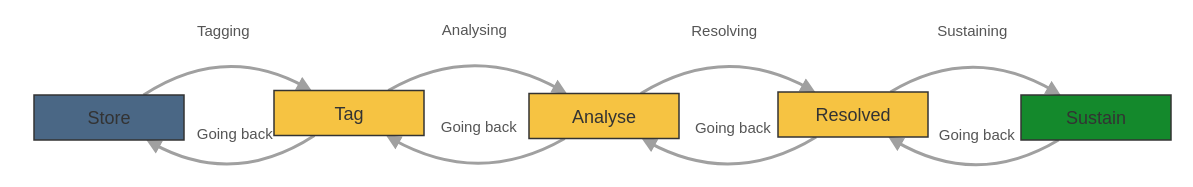
\includegraphics[width=6.535in]{workflow_stars.png}
\caption{Procédure STARS dans l'application Projet vue Diagramme}
\label{fig:workflow_stars}
\end{figure}

Ainsi, on peut créer un nouveau projet et suivre cette procédure en ajoutant des tâches d'amélioration continue de son organisation, voir Figure~\ref{fig:kanban_stars}.

\begin{figure}
\centering
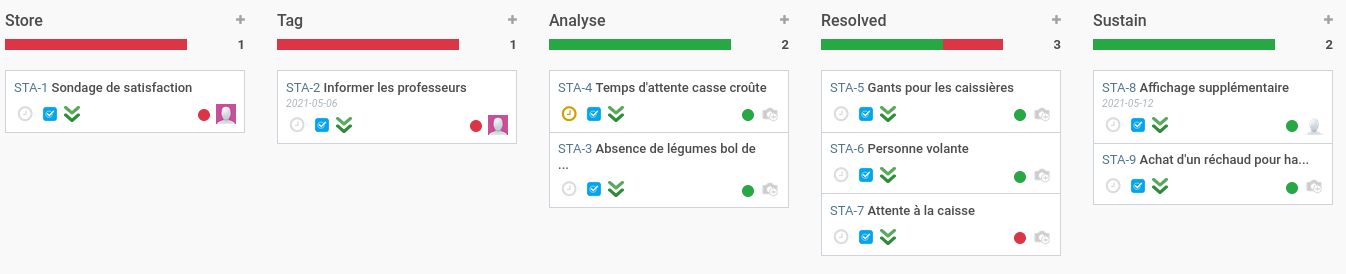
\includegraphics[width=6.535in]{kanban_stars.png}
\caption{Suivi des tâches de projet avec procédure STARS en vue Kanban}
\label{fig:kanban_stars}
\end{figure}

\subsection{Projet module SRS}

C’est un module de gestion de projet généré par le générateur de code qui permet de faire l’analyse des besoins pour ensuite passer à l’analyse fonctionnelle et finalement définir les requis fonctionnelles d’un projet. Il a été utilisé en autre pour le projet Accorderie et le projet Portail CEPPP.

\section{Projet espace Accorderie}

Le projet a débuté par l'élaboration d'une analyse des besoins et fonctionnelles, puis un ensemble de requis logicielles ont été rédigé avec un membre du Réseau de l'Accorderie. % TODO faire annexe, voir annexe OIU.

Le générateur de code a permis créer un module Odoo 12.0 avec leurs modèles de données basé sur leur base de données en \texttt{SQL} de MariadB, voir Annexe~\ref{annexe_db_accorderie_2019}.

Plusieurs corrections ont été effectué avant la migration : correction des noms des champs pour les uniformisés; correction des types de champs (exemple le «True» était exprimé par la valeur «-1» dans un type «int», ainsi ce type a été transformé en booléen); enlever les double dépendances par changement de l’architecture; correction des données erronés (un champs est requis, mais il manque des données pour certaines entrées). De plus, le modèle de données n’a pas été conçue pour de l’automatisation, mais plutôt pour que les échanges de service soient validés par des membres de la communauté.

Dans l'Annexe~\ref{annexe_db_accorderie_2023}, on peut observer les adaptations des champs. Par exemple, avec la table «accorderie\_echange\_service», il y a l'ajout des champs : «nb\_heure\_estime» pour avoir une prévision des heures à effectuer, «nb\_heure\_dure\_trajet» pour reconnaître le temps de déplacement, «distance\_trajet» pour connaître la distance qui sera calculé avec le projet libre \texttt{OSRM}, etc...

La migration du modèle de données a été faite dans un module qui dépend de la technique «Migration DB» qui permet d'importer le modèle. Certaines données nécessitent la création d’un fichier de données \texttt{XML}. Pour les autres données, un autre module a été créé pour ajouter les données directement dans une base de données qui sera migré vers une mise en production.

Un portail a été généré, pour remplacer les formulaires utilisés par l'ancienne plateforme \texttt{PHP} et ainsi visualiser les entrées. Cependant, cette fonctionnalité a été abandonné puisque cette technologie ne plaisait pas

Une maquette a été conçue pour un nouvel espace membre. Ainsi, on a utilisé la technique «website\_snippet» pour afficher des données sur le site web et créer des formulaires. Cette base a permis d’accélérer la création de code de communication entre le client et le serveur. À force de faire l’intégration et la personnalisation de cette maquette, il n’y a plus vraiment de code qui provient du générateur de code.

Le générateur de code a permis d’aider à créer un diagramme pour afficher le processus d’échange de temps, voir Annexe~\ref{annexe_processus_accorderie_2023}, puis une application en Javascript avec AngularJS a été développé pour afficher ce processus à l’utilisateur, une machine à état qui permet de revenir selon des paramètres à un état du processus.

Dû à des limitations humaines et de temps, tout le reste du projet a dû être fait manuellement puisqu’on a changé de technologie pour faciliter le développement de l’interface.

\section{Projet Portail CEPPP}

L'objectif est de faire une section portail pour les patients et une section administratif pour les recruteurs, les partenaires et les administrateurs de la plateforme, rendre accessible des formulaires et anonymiser les données. Le mandat était de migrer les fonctionnalités de la plateforme qui a été développé sur SuiteCRM en \texttt{PHP}.

Un module d'extraction de \texttt{PHP} a été développé, mais il n'est pas accessible dans les techniques du générateur de code. Le modèle de données était directement dans le code puisqu'il est dynamique, il n'est pas dans la base de données. La base de données n'a pas été extraite, les données ont été exporté en \texttt{CSV} et un module d'exportation des données a été développé.

Extraction : 
\begin{enumerate}
    \item 23 fichiers analysés;
    \item 2851 données extraites;
    \item Capacité de faire la traduction anglais-français sur les données, mais cette fonctionnalité annulé puisque les données ont été modifié dans la ré-ingénierie.
\end{enumerate}

Voici les statistiques~\ref{tab:stat_code_portail_ceppp} du code après ré-ingénierie et adaptation des fonctionnalités, livraison de la plateforme en début septembre 2023\footnote{\url{https://portailppp.ca}}.

\begin{table}[htb]
\caption{L'évolution entre la génération et la ré-ingénierie des statistiques sur les langages du portail CEPPP}
\centering
\begin{tabular}{|l|l|l|l|}

\hline
\cellcolor[HTML]{d9d9d9}{\textbf{Langage}} & \cellcolor[HTML]{d9d9d9}{\# Ligne extrait} & \cellcolor[HTML]{d9d9d9}{\# Ligne personnalisé} & \cellcolor[HTML]{d9d9d9}{\# Diff}\\\hline

\texttt{XML} & 6 861 & 3 856 & - 3 005\\\hline
Python & 567 & 1 564 & + 997\\\hline
Javascript & 0 & 68 & + 68\\\hline
\texttt{CSV} & 25 & 51 & + 26\\\hline

\end{tabular}
\label{tab:stat_code_portail_ceppp}
\end{table}

L'anonymisation n'est pas supporté par le générateur de code, puis la personnalisation enlève beaucoup de champs mis de manière générique dans les fichier \texttt{XML}. 

Le modèle de données du portail CEPPP dans Odoo 12 contient 24 modèles~\ref{annexe_db_ceppp_2022}. L'interface administrateur~\ref{annexe_form_ceppp_2022} contient la fiche du patient, que les partenaires ont accès seulement qu'à la partie anonymisée~\ref{annexe_form_anonyme_ceppp_2022}.

